      
               
                \begin{ledgroupsized}[r]{120mm}
                \footnotesize 
                \pstart                
                \noindent\textbf{\"{U}berlieferung:}   
                \pend
                \end{ledgroupsized}
            
              
                            \begin{ledgroupsized}[r]{114mm}
                            \footnotesize 
                            \pstart \parindent -6mm
                            \makebox[6mm][l]{\textit{L}}Konzept: LH XXXV 3A, 16 Bl. 19\textendash20. 1 Bog. 2\textsuperscript{o}. 2/3 S. Verbleibender Teil von Bl. 19 r\textsuperscript{o} sowie Bl. 19 v\textsuperscript{o}, 20 r\textsuperscript{o} und 20 v\textsuperscript{o} \textit{LSB} VII, 1 N. 57. In der oberen Seitenh\"{a}lfte die ersten acht Zeichnungen unseres Textes. Die neunte Zeichnung Seitenmitte rechts. Daneben links Rechnungen aus \textit{LSB} VII, 1 N. 57, die auf den letzten 3 Zeilen fortgesetzt werden.\\Cc 2, Nr. 718 \pend
                            \end{ledgroupsized}
                %\normalsize
                \vspace*{5mm}
                \begin{ledgroup}
                \footnotesize 
                \pstart
            \noindent\footnotesize{\textbf{Datierungsgr\"{u}nde}: Unser St\"{u}ck befindet sich auf einem Bogen, der den Text \textit{LSB} VII, 1 N. 57 enth\"{a}lt. Das Wasserzeichen des Texttr\"{a}gers ist f\"{u}r die Zeit August\textendash September 1674 gut nachgewiesen. Wir \"{u}bernehmen die Datierung des genannten Textes aus Reihe VII.}
                \pend
                \end{ledgroup}
            
                \vspace*{8mm}
                \pstart 
                \normalsize
            [19 r\textsuperscript{o}] Post ablationem obicis \edtext{totum spatium}{\lemma{obicis}\Afootnote{ \textit{ (1) }\ omnia \textit{ (2) }\ totum spatium \textit{ L}}} simul descendunt, 
            $\displaystyle \frac{b}{a}\sqcap \frac{3}{1}\rule[-4mm]{0mm}{10mm} $
        %    $\displaystyle 1\frac{1}{3}\rule[-4mm]{0mm}{10mm} $
             actio in linea \textit{b} erit ad actionem in linea \textit{a},  comme \textit{a} ad \textit{b}, id est ut $\displaystyle \frac{1}{3}\rule[-4mm]{0mm}{10mm} $. Non potest augeri celeritas, quia deberet exire celerius columna perpendicularis,  intermedia. Atqui columna perpendicularis non potest celerius  quam postulat\edtext{}{\lemma{}\Afootnote{postulat  \textbar\ ejus \textit{streicht Hrsg.}\ \textbar\ gravitas \textit{ L}}} gravitas ejus propria.\pend \pstart  Nihil probatur major, quia nihil potest exire nisi exeat  prius aliquid columnae intermediae.\pend \pstart  Nam si posset aliquid exire praeter columnam interm[ediam].  Nihil ex columnis lateralibus exire potest ante mediam.  Nam conatus columnarum lateralium impeditur aut  probetur. Nam columna intermedia \edtext{imp}{\lemma{intermedia}\Afootnote{ \textit{ (1) }\ agit contra \textit{ (2) }\ imp \textit{ L}}} [\textit{Satz bricht ab}]\footnote{\textit{Rechts neben [Fig. 8]}:  $\displaystyle 1\frac{1}{3}$}  \pend
% Zeitz auskommentiert          %  \begin{center}
%                  %    \includegraphics[width=0.4\textwidth]{images/35_3A_19r1}
%                     % \includegraphics[width=0.2\textwidth]{images/35_3A_19r2}
%                      %\includegraphics[width=0.2\textwidth]{images/35_3A_19r3}\\
%                      %\includegraphics[width=0.2\textwidth]{images/35_3A_19r4}
%                      %\includegraphics[width=0.2\textwidth]{images/35_3A_19r5}
%                      %\includegraphics[width=0.2\textwidth]{images/35_3A_19r6}
%                      %\includegraphics[width=0.2\textwidth]{images/35_3A_19r7}
%                      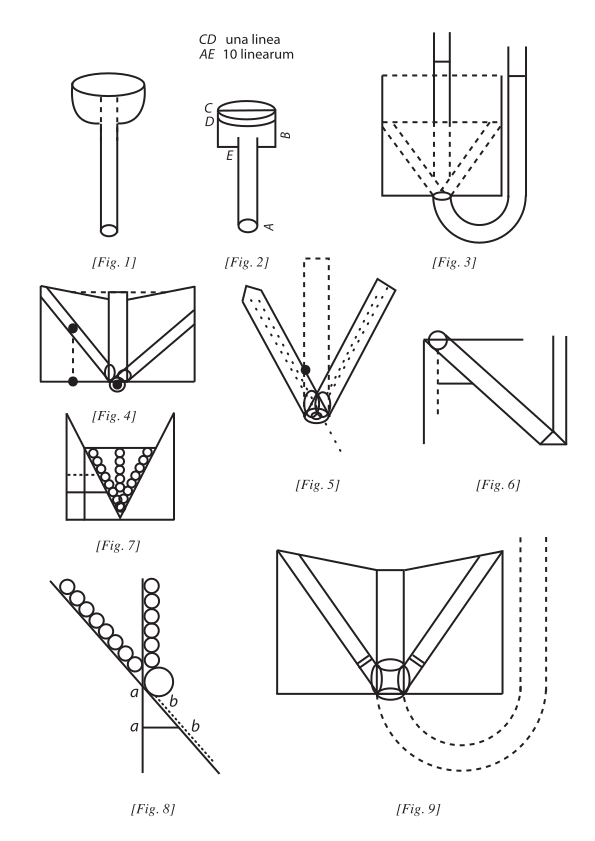
\includegraphics[width=0.9\textwidth]{images/35_3A_19r_gesamt}
%               %       \end{center}
                      